\section{融合图片信息的神经机器翻译}
\label{sec:2_imgnmt}

%研究意义与背景介绍
得益于深度学习技术在自然语言理解和计算机视觉等领域的快速发展,融合文本与图片信息的跨模态理解与生成也成为了可能。融合图片信息的神经机器翻译就是将已经成熟的计算机视觉方法与神经机器翻译技术相结合的一个研究方向。其研究历程也紧随着纯文本神经机器翻译的脚步而发展。一个标准的神经机器翻译系统通常以句子为翻译单位。端到端的翻译模型通过拟合大量双语数据中语言之间的对齐特性习得翻译能力,在编码过程将源语言句子的信息编码为分布式的向量表示,再通过解码器将表示向量解码到目标语言。然而,针对翻译采集的数据也包含着人类语言在应用中所保留的使用习惯与问题。例如文本中存在多译词、歧义词或者不完整表达等问题,都需要通过待翻译句子以外的补充信息解决,而图片中往往包含着更丰富、更完整或者更准确的额外信息。因此在翻译一个句子时,图片信息能够为其提供所需的外源补充信息。为此,研究者们提出了融合图片信息的神经机器翻译方法(image-incorporated neural machine translation,ImgNMT)。

% 任务定义
融合图片信息的神经机器翻译方法的目的是在基于神经机器翻译的框架内,借助图片信息生成更准确的译文。该方法是多模态机器翻译(multi-modal machine translation)的一个研究子类。相关的多模态机器翻译还包含口语翻译\pcite{vida1997finite,ney1999speech,weiss2017sequence,berard2018end}(spoken language translation,SLT)和视频引导翻译\pcite{lison2016opensubtitles2016,sanabria2018how2,wang2019vatex}(video-guided translation,VGT)\pcite{sulubacak2020multimodal}。目前已知的多模态翻译方法多数是融合了两个模态信息的跨模态方法。视频引导翻译与融合图片信息的翻译任务有着相似的特点,都是在文本翻译的基础上通过融合视觉信息提升翻译性能,但也因此相关研究较少。

% 研究方法及其分类
作为多模态机器翻译领域的一个重要方向,ImgNMT得到了学界的广泛关注。2016年机器翻译研讨会(workshop on machine translation,WMT)开展多模态机器翻译的相关评测\pcite{specia2016shared},彼时的多模态机器翻译任务的目标是为图片生成目标语言的译文,因此可分为两种解决方案:第一种是利用图片信息生成目标语言句子,这种任务形式一般称为图像描述生成(image captioning)或图像翻译;另一种就是在文本翻译任务中加入图片信息辅助翻译过程,也就是本文关注的ImgNMT。在此之后,WMT 2017\pcite{elliott2017findings}和WMT 2018\pcite{barrault2018findings}将多模态机器翻译的研究进一步推向全世界,越来越多的相关研究相继涌现。本节对融合图片信息的神经机器翻译的国内外研究现状进行了系统的梳理和分类。本文将相关研究分为四个类别:图片信息辅助式神经机器翻译、图片信息增强式神经机器翻译、基于图片搜索的神经机器翻译以及基于图片信息的无监督神经机器翻译,并分别在后续的小节中进行详细的介绍。

%得益于神经网络方法的快速发展,自然语言文本与图片的信息融合成为了可能。融入图片信息的机器翻译的研究历程也紧随着纯文本的神经机器翻译的脚步而发展。然而,相关研究则最早起源于图像描述生成任务。有部分学者将文本作为一个外源信息来辅助图片描述的生成,但这种方式的本质则是在翻译任务中融入视觉信息。2016年WMT将多模态机器翻译引入作为共享任务后,MMT受到了广泛的关注。在之后的WMT17和WMT18,MMT任务延续并奠定了在机器翻译中融合图片信息作为多模态机器翻译研究的主要范式。

%平行翻译句一般具有良好的对齐特性,这使得融入的外源信息仅用于辅助少数具有歧义、信息不完整以及训练不充分等问题的句子的翻译。该特性也成为了展开相关研究道路上的一大难点。
%融合图片信息的神经机器翻译任务主要采用的是平行翻译句对加图片三元组形式的数据,即一张图片对应一句描述和一句翻译。大部分相关研究需要对神经机器翻译模型进行适当的修改,以适应图片的输入。模型中输入的图片可用于辅助优化翻译过程中源语言的语义表示,或为解码过程增加辅助外源信息。本文将这种在翻译过程中以源端文本作为信息主体,输入图片用于语义信息强化的方法称为图片信息辅助式神经机器翻译。可根据图片信息融合到翻译模型中的方式将这种方法分为三类:融合图片全局信息、融合图片局部动态信息以及融合图片视觉目标信息。这些三种图片信息以视觉特征为载体输入到翻译模型中,视觉特征则是从预训练的卷积神经网络中提取得到。不同的提取方式所包含的语义信息的粒度和特征维度有所不同。将这些不同形式的视觉特征整合到NMT模型后,模型进行跨模态语义融合的难易程度则取决于模型设计的合理性。


%以下两种方式合并讨论:
% 还可分为编码融合方法,和解码融合方法
% 全局 局部 视觉目标

% 显式、隐式:放到最后与igt和iet交叉讨论
% 这个章节中可以多提一下ImgNMT与多模态摘要任务的区别
\subsection{图片信息辅助式神经机器翻译}
\label{sec:2_ignmt}
\begin{figure}[!htbp]
    \centering
    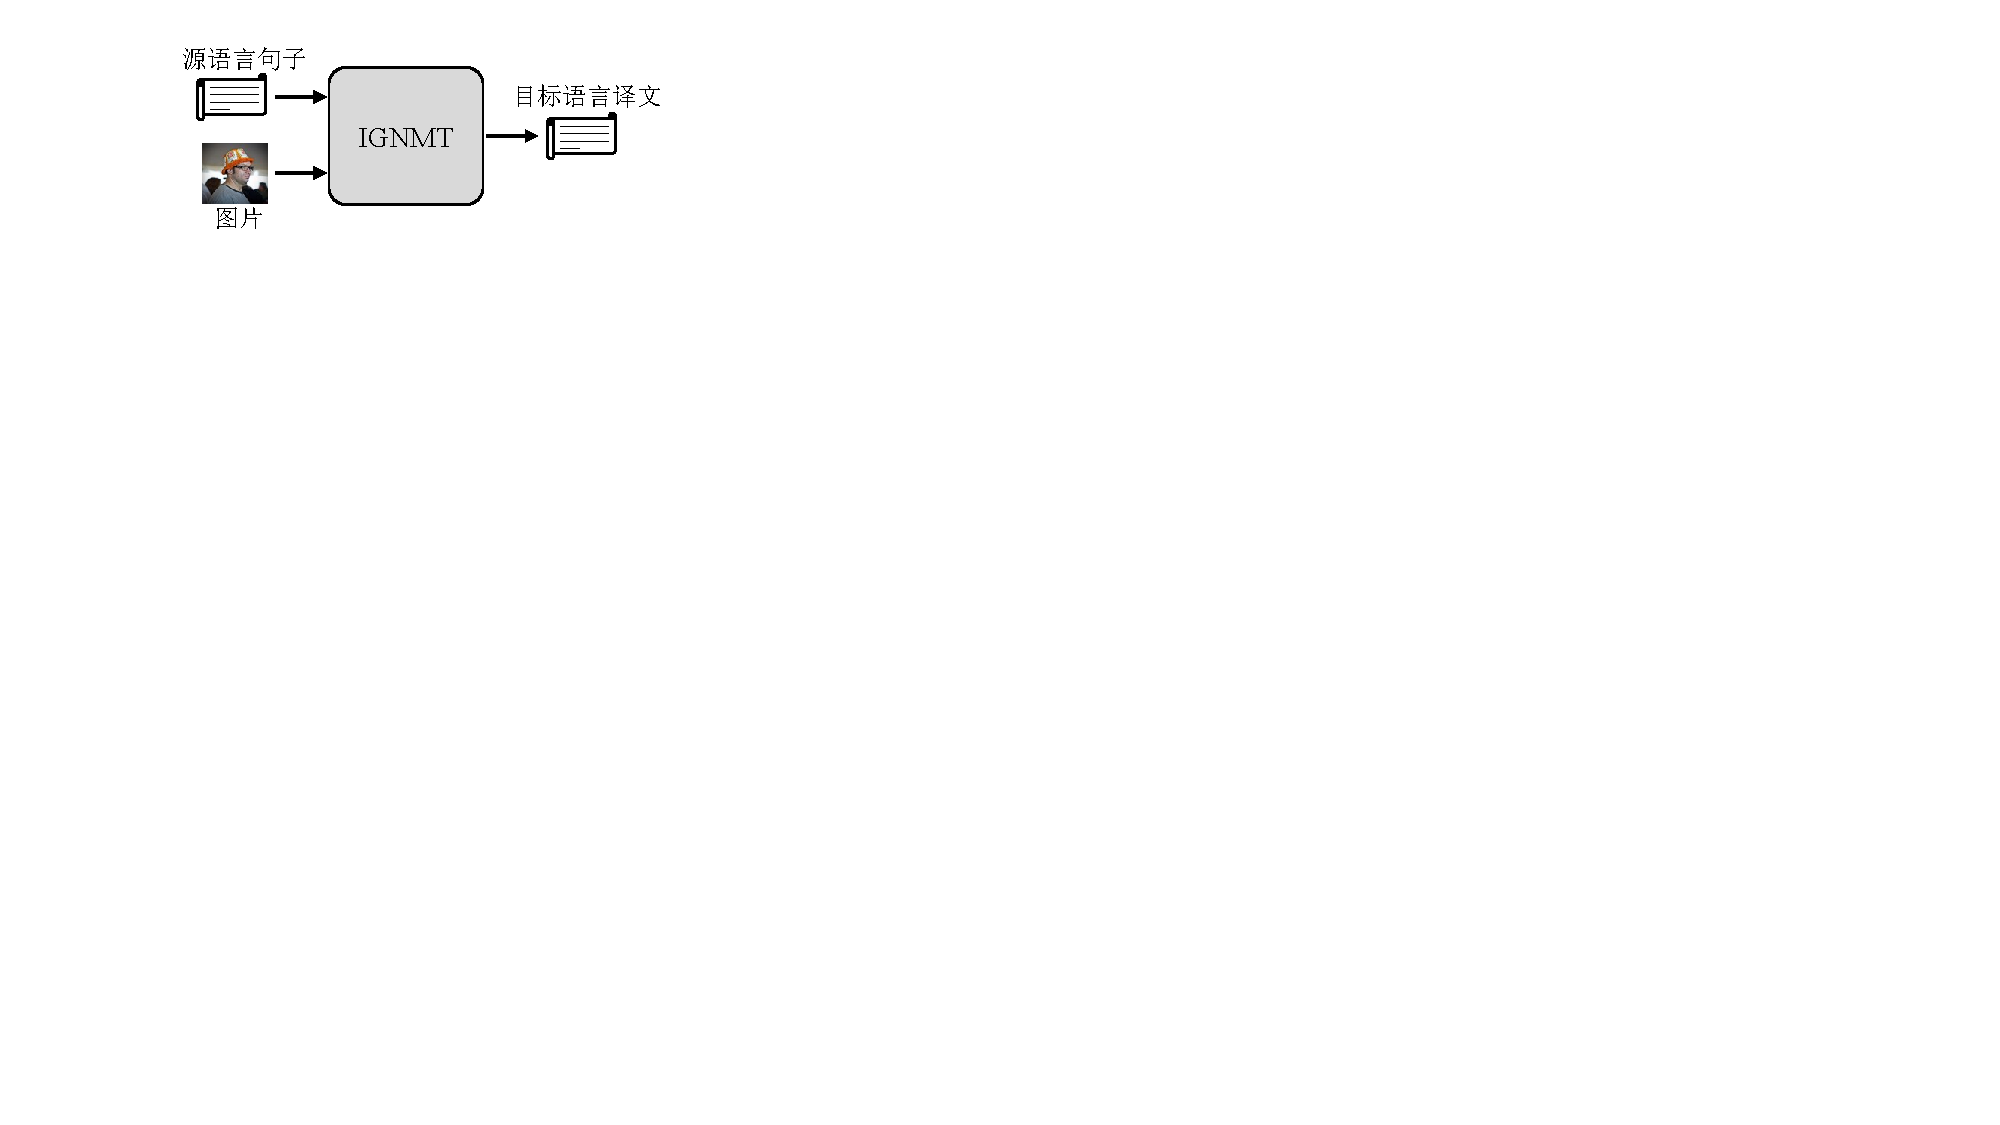
\includegraphics[scale=1]{Img/fig_2_ignmt.pdf}
    \bicaption{图片信息辅助式神经机器翻译}{Image-guided neural machine translation}
    \label{fig:2_ignmt}
\end{figure}
图片信息辅助式神经机器翻译方法又称图片引导式神经机器翻译方法(image-guided neural machine translation,IGNMT),是融合图片信息的神经机器翻译方法中最常见的一类分支,也是融合图片信息最自然的一类方法,理论上还是视觉信息利用程度最高的一类方法。这类方法的特点是将图片直接输入到翻译模型中,通过直接的模型学习或某种人为设计的方式,使翻译模型在进行编码源语言句子或解码目标语言句子时,通过利用输入的图片信息完成更好的编码表示或进行更准确的解码生成,从而得到更准确的译文。因采用编码器-解码器结构的翻译模型具有非常灵活的使用方式,同时在\ref{sec:2_cv}节中提到,图片特征的提取方式也分为多种,所以将图片信息融合到翻译模型中的方法也有很多。本节将这些方法从两个方面进行分类,从作用到翻译模型结构中的不同组成部分可分为:编码融合方式和解码融合方式;从图片的视觉特征使用方式的不同可分为:全局特征融合方法、局部特征融合方法以及视觉目标特征融合方法。

\subsubsection{基于模型结构的图片信息融合方法}

{\sffamily (1)编码融合}

基于编码器-解码器结构的神经翻译模型中,编码器负责将源语言句子编码为向量表示。在编码前,源语言句子中的单词会被转换成利用分布式向量表示的词向量。在编码过程中,分散在输入序列的信息将通过循环神经网络或多头自注意力机制按照序列内各项的位置信息交织并融合,序列中每一项的特征向量不再是一个单独的表示,而代表着融合了句子中上下文信息的向量表示。在编码后,句子的隐层向量表示将传递给解码器用于解码目标语言。在编码的前、中、后三个阶段,均是图片信息可以参与的阶段。

\tcite{calixto2017incorporating}尝试在编码前,将图片的全局特征以前、后以及两侧三种方式与源语言句子词向量序列拼接,然后将图片信息融合到源语言句子的编码中。\tcite{huang2016attention}提出了另外两种方案,一是利用R-CNN提取出图片中视觉目标的全局特征,然后连同完整图片的全局特征作为序列拼接到文本输入前,最后利用编码器一起编码;二是将每个视觉目标单独拼接到文本序列前,然后对每个这样的序列都进行一次单独的编码,在解码的过程中需要通过注意力机制选择与当前解码状态最相关的那个编码序列。为了使模型更充分地学习跨模态信息的融合,还可以采用大规模视觉语言预训练模型(vision-language pre-trained model)的方案\pcite{caglayan2021crosslingual,wang2021make,susanto2021rakutens,yawei2021probing,hirasawa2022pretrained}。这种方法主要利用更大规模的数据和更多模型参数的优势使模型具备更强的跨模态信息融合能力,其模型多是基于Transformer结构,模型的输入是句子和图片的组合方式。不难看出,虽然各类方法在编码前阶段就需要将图片与文本拼接到一起,但该过程并不能起到信息的融合作用,仅影响了图片在模型编码过程中的作用方式。这些方法的跨模态信息融合过程依赖的是循环神经网络或基于自注意力机制的Transformer编码器所具备的序列建模能力。

在编码前将图片和句子组合的方式具有方法简单的优点,但通常也会增加模型的学习难度。因此,有相关工作尝试利用模型或数据的特点,通过设计模型的使用方式或模型结构,使模型在编码的过程中融合图片信息。最早的相关工作利用图片的全局特征初始化基于循环神经网络的编码器的初始状态\pcite{elliott2015multilanguage,calixto2017doubly}。\tcite{yang2020visual}在编码的过程中通过建立视觉目标特征序列和文本表示序列的相似度矩阵,得到文本序列与视觉目标序列之间的相似度,并在进一步的文本表示编码中将相似度作为注意力值加权计算,最后为了提升图片信息的作用,在训练过程中加入了正则化损失。\tcite{yin2020novel}采用了图结构建模源语言句子与图片中视觉目标的关系,然后设计了基于多头注意力机制的面向图结构的多模态编码器,在编码的过程中将视觉目标节点和文本单词的节点单独编码,然后再用交叉注意力机制获得单词节点的视觉目标特征表示和视觉目标特征的单词表示,最后将文本节点的编码结果传递给一个常规的解码器。

在翻译的编码过程完成后再进行视觉信息融合的方法相当于利用图片对文本表示进行二次编码。\tcite{wang2021efficient}在文本编码器得到隐层表示后,增加了视觉目标与源语言句子之间的关联表示。该方法设计了以多头注意力为基础的目标-源注意力层(object-source attention layer),建立文本序列的视觉目标表示,并在损失函数中加入了目标掩码损失函数使模型更多的关注与源语言信息相关的视觉目标。\tcite{wu2021good}和\tcite{li2021vision}都在编码后采用了门控机制,利用图片的全局特征与文本向量表示语义关系,建立能够控制图片全局特征编码参与度的门控向量,最后将门控向量作用到文本的隐层向量与图片全局特征的加权和上。

{\sffamily (2)解码融合}

基于编码器-解码器结构的神经翻译模型中,解码器负责将编码过的文本向量表示解码到目标语言。而该过程是自回归解码(autoregressive decoding),即解码目标语言句子时每个时间步只能生成一个单词,每个单词的生成需要依赖前面的解码时间步和源语言所提供的信息。源语言提供了整个句子的完整的静态信息,前面时间步已经解码的结果为解码器提供当前时间步需要哪些动态信息。从解码器的工作方式不难看出,图片在解码过程中的主要作用与源语言句子类似,提供的是静态信息。
与编码器类似,早期方法将图片的全局特征作为完整的视觉语义信息用于初始化基于循环神经网络的解码器的初始状态,从而在解码的循环迭代中,在隐层向量中保留着图片所提供的信息\pcite{elliott2015multilanguage,calixto2017incorporating,zhou2018visual,zheng2018ensemble}。

然而,这种利用图片特征初始化循环神经网络的方式在解码过程中存在遗忘的问题。在解码到后面的单词时,隐层表示中所保留的视觉信息将越来越少,因此这种视觉信息作用方式的效果很有限。除此之外,这种方法仅适用于基于循环神经网络的方法,无法适用于更广泛应用的基于Transformer的神经机器翻译。注意力机制在出现后成为解决这类问题最受欢迎的解决方案。
早期基于循环神经网络的神经机器翻译模型采用了增加图片注意力模块的方式\pcite{caglayan2016multimodal,calixto2017doubly,caglayan2018liumcvc,gain2021iitp,laskar2021improved}。图片注意力模块的实际工作方式与文本注意力模块是相似的,可以根据当前解码状态判断图片的栅格特征中哪些区域的视觉信息对于解码当前步的单词是有用的。因此这种方法能够为解码器提供动态的图片局部信息。
\tcite{zhao2020double,zhao2021tmeku}同样采用了双注意力机制的方案,不同的是,该方法提供的是从Faster R-CNN中提取的视觉目标序列。
在基于Transformer的神经机器翻译模型的解码器中,一般采用的是增加针对图片的交叉注意力模块\pcite{arslan2018doubly,gronroos2018memad,libovicky2018input}。
\tcite{liu2021gumbel}认为这些方法很难使模型注意到图片中的有用信息,并且会引入大量的噪音,因此使用了Gumbel-Softmax改造了注意力机制。
\tcite{li2022vision}所提方法并没有采用从卷积神经网络提取出来的图片特征,而是采用了ViT(vision Transformer)\pcite{liu2021swin}模型提取出来的图片特征,然后利用交叉注意力机制和门控机制的组合方式,为解码器提供图片信息。
注意力机制不仅可以在解码过程中使用,同样可以应用于解码后。\tcite{ive2019distilling}在解码器后端增加了用于二次解码的推敲网络(deliberation network),同样使用了注意力机制,并且可以关注源语言信息、视觉目标信息以及第一次的解码信息。

\subsubsection{基于图片特征结构的图片信息融合方法}
在前面的\ref{sec:2_cv}节中介绍到,直接从卷积神经网络中可以提取到全局特征和栅格特征。利用目标检测方法可以提取出图片中最具有前景信息价值的视觉目标。本节,我们根据这些图片特征的特点,对现有的融合图片信息的神经机器翻译方法进行分类。

{\sffamily (1)图片栅格特征}

图片栅格特征一般提取自卷神经网络全连接层之前的输出,例如\tcite{calixto2017doubly}所提方法采用的就是ResNet-50\pcite{he2016deep}全连接层之前非线性激活层的输出。在连入全连接层之前,卷积神经网络对图片进行编码的过程一直保留着图片的二维信息,例如一个大小为$224 \times 224$的图片经过ResNet-50编码得到一个$7 \times 7 \times 2048$的特征表示。其中$7 \times 7$的矩阵将原图片分为49个区域并一一对应,因此这个特征表示可以看做是对图片中49个区域的编码,每个编码的维度是2048。从这种表示方法不难看出,图片栅格特征可以当作对图片编码后产生的编码序列,这个序列的长度为49。在上一小节中介绍的方法中,多数使用注意力机制的方法都应用了图片的栅格特征,并以图片特征序列的形式输入到翻译模型中。与文本序列不同的是,这种形式的图片输入序列的长度是固定的。虽然栅格特征尽可能地保留了图片中的信息,还可以当做图片序列方便模型的设计,但是也存在着一定缺点。一是栅格特征尽可能保留信息的同时也保存了大量与文本翻译不相关的噪音信息,\tcite{liu2021gumbel}就是在这个原因的基础上设计的Gumbel注意力机制。二是这种图片序列与文本序列最大的不同并不是序列的长度是否固定,而是图片中的内容往往更随意,但文本序列满足一定的语法规律。例如图片中的人物可以出现在图片中的任何位置,或者将图片旋转或倒置都不会改变图片内部的主要信息,但是这种操作会对图片信息在栅格特征中的表征位置带来影响\pcite{azulay2019why,kim2020cycnn,mo2022riccnn},最终影响到序列中的位置。这说明了相比于文本序列,图片栅格特征序列所包含信息的位置更随意,使翻译模型难以根据语义信息直接定位到有效信息在栅格特征中的位置。

{\sffamily (2)图片全局特征}

图片全局特征一般来自于将图片的栅格特征经过平均池化层得到的单个表征向量,也可以选择卷积神经网络全连接层的输出向量。例如将ResNet-50的栅格特征经过平均池化后得到一个2048维的图片特征向量,或者像\tcite{calixto2017incorporating}一样采用VGG19\pcite{simonyan2015very}的全连接层输出向量。相比于图片栅格特征,这种全局特征可以看做同样保留了图片完整语义信息。其作用方式与早期基于循环神经网络的神经机器翻译模型用编码器的最后一个隐层向量解码到目标语言类似,同样是利用单个特征向量表征完整的语义。但因为是单个特征向量,所以图片全局特征丢失了图片中的二维空间信息。然而,图片全局特征也有着栅格特征所不具备的优点。一是单个特征的方式更容易嵌入到神经机器翻译模型中,甚至不需要对翻译模型做改动,例如,可以作为词向量或用于初始化模型。二是可以避免卷积神经网络不具备旋转不变性(rotation invariance)带来的问题。

{\sffamily (3)视觉目标特征}

视觉目标特征的提取一般采用目标检测方法提取到视觉目标后,再使用卷积神经网络提取视觉目标的全局特征,或者直接使用目标检测方法自带的卷积神经网络在检测过程中输出视觉目标的全局特征。在使用的数据已有视觉目标的标注情况下,也可以直接将图片中的视觉目标区域裁剪出来,再提取其全局特征。采用视觉目标特征时,通常不使用视觉目标的栅格特征。这是因为视觉目标的信息比完整图片所包含的信息更集中也更明确,并且一般集中于图片中的单个目标。所以多数情况下没有必要保留视觉目标的二维空间信息。视觉目标特征的优点就是在目标提取过程中为每个目标过滤掉了背景信息,使所采用的视觉信息更集中于图片中的关键信息。并且,一张图一般可以提取出多个视觉目标,这些视觉目标可以以排成序列的形式输送给翻译模型。视觉目标特征同样存在着缺点。一是目前的目标检测算法的检测结果与真实的目标区域仍存在着一定的偏差,提取的视觉目标可能并不准确,或仍保留大量的噪音。二是虽然这种方式能够过滤掉背景信息,但也存在着过滤掉有用信息的可能。为了避免这些问题对神经机器翻译模型造成影响,一般采用输入视觉目标特征的同时,也输入完整图片的全局特征\pcite{huang2016attention,ive2019distilling,ive2021exploiting,wang2021efficient}。


%得益于神经网络方法的快速发展,自然语言文本与图片的信息融合成为了可能。融入图片信息的机器翻译的研究历程也紧随着纯文本的神经机器翻译的脚步而发展。然而,相关研究则最早起源于图像描述生成任务。有部分学者将文本作为一个外源信息来辅助图片描述的生成,但这种方式的本质则是在翻译任务中融入视觉信息。2016年WMT将多模态机器翻译引入作为共享任务后,MMT受到了广泛的关注。在之后的WMT17和WMT18,MMT任务延续并奠定了在机器翻译中融合图片信息作为多模态机器翻译研究的主要范式。

%平行翻译句一般具有良好的对齐特性,这使得融入的外源信息仅用于辅助少数具有歧义、信息不完整以及训练不充分等问题的句子的翻译。该特性也成为了展开相关研究道路上的一大难点。
%融合图片信息的神经机器翻译任务主要采用的是平行翻译句对加图片三元组形式的数据,即一张图片对应一句描述和一句翻译。大部分相关研究需要对神经机器翻译模型进行适当的修改,以适应图片的输入。模型中输入的图片可用于辅助优化翻译过程中源语言的语义表示,或为解码过程增加辅助外源信息。本文将这种在翻译过程中以源端文本作为信息主体,输入图片用于语义信息强化的方法称为图片信息辅助式神经机器翻译。可根据图片信息融合到翻译模型中的方式将这种方法分为三类:融合图片全局信息、融合图片局部动态信息以及融合图片视觉目标信息。这些三种图片信息以视觉特征为载体输入到翻译模型中,视觉特征则是从预训练的卷积神经网络中提取得到。不同的提取方式所包含的语义信息的粒度和特征维度有所不同。将这些不同形式的视觉特征整合到NMT模型后,模型进行跨模态语义融合的难易程度则取决于模型设计的合理性。

%\subsubsection{融合图片全局信息的神经机器翻译}


%\subsubsection{融合图片局部动态信息的神经机器翻译}

%\subsubsection{融合图片视觉目标信息的神经机器翻译}



\subsection{图片信息增强式神经机器翻译}
% 这类方法特点不是为了解决语料中自带问题,例如歧义词,而是为了解决模型在训练过程中存在的问题,算是两种不同的思路

\begin{figure}[!htbp]
    \centering
    \begin{subfigure}{0.5\textwidth}
      \centering{
      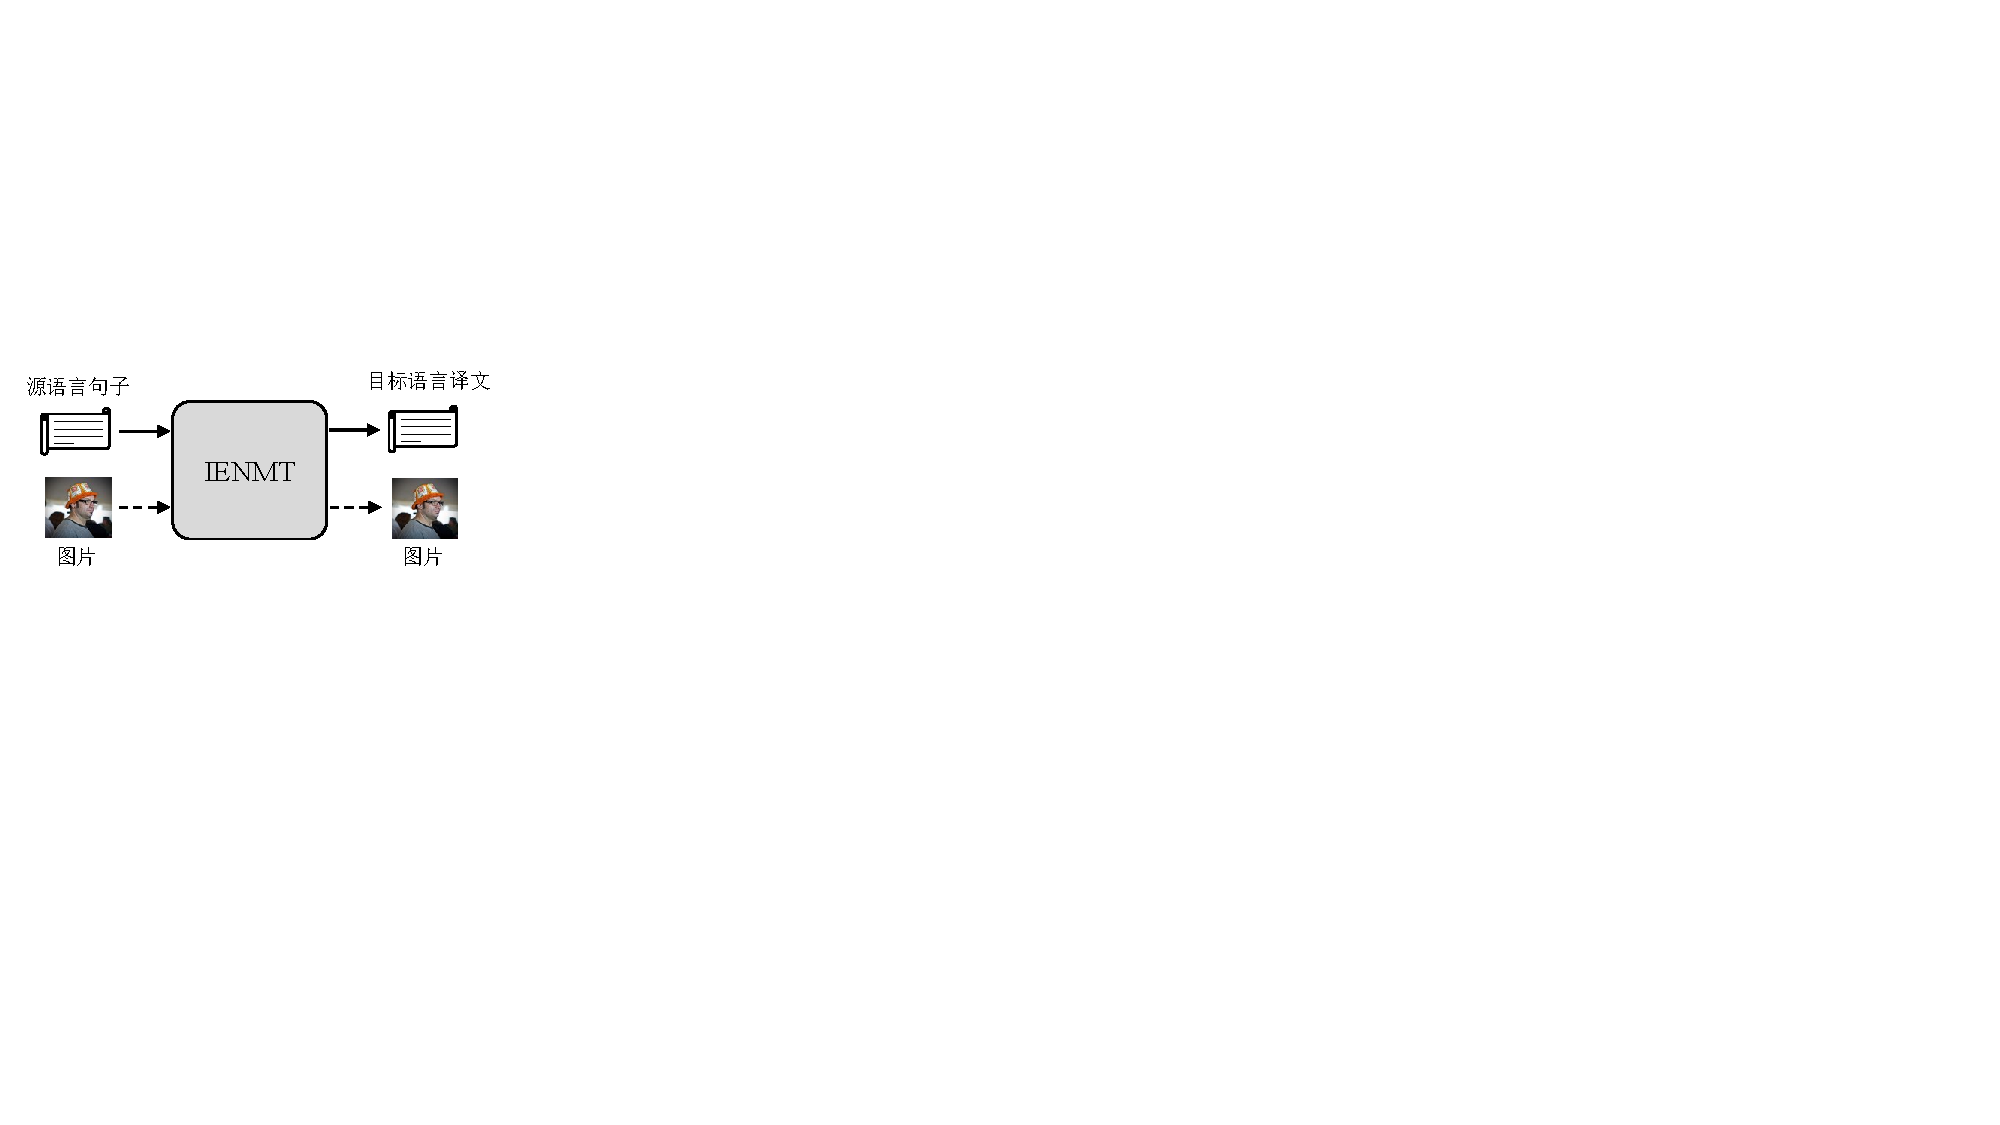
\includegraphics[width=\textwidth]{Img/fig_2_ienmt_train.pdf}
      \caption{训练阶段}
      \label{fig:2_ienmt_train}}
    \end{subfigure}%
    ~% line break
    \begin{subfigure}[b]{0.5\textwidth}
      \centering
      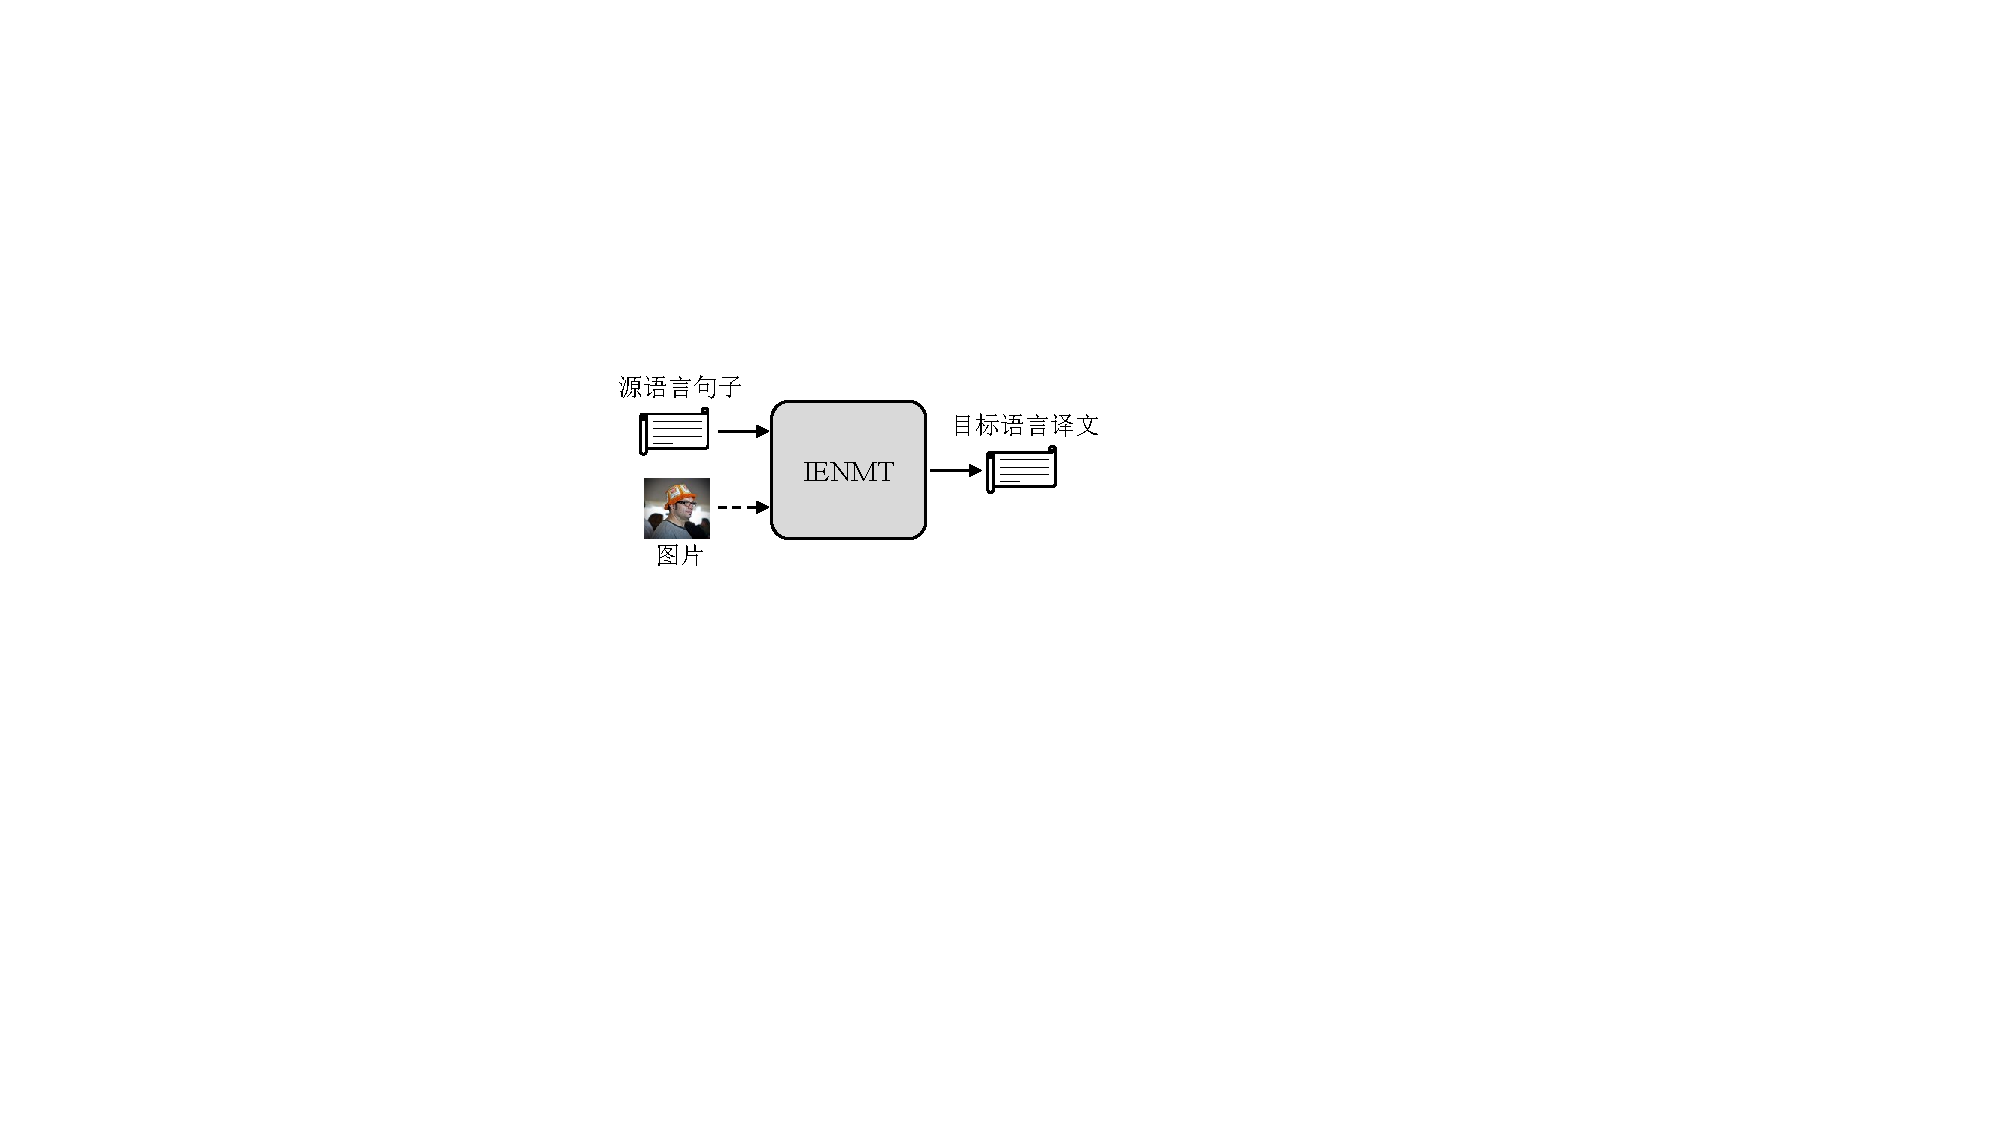
\includegraphics[width=\textwidth]{Img/fig_2_ienmt_infer.pdf}
      \caption{测试阶段}
      \label{fig:2_ienmt_infer}
    \end{subfigure}
    \bicaption{图片信息增强式神经机器翻译}{Image-enhanced neural machine translation}
    \label{fig:2_ienmt}
\end{figure}
上一节所述的图片信息辅助式神经机器翻译的主要特点是需要将图片输入到模型中,是模型利用视觉信息辅助整个翻译过程。期望通过这种方式解决待翻译文本中存在的多种病句问题,并且有大量的研究工作在这种方法范式上展开。然而,图片的作用方式不仅如此。图片信息增强式神经机器翻译(image-enhanced neural machine translation,IENMT)是一种利用特定的作用方式,将图片信息作用到模型的训练优化过程中,使神经机器翻译模型受益于这种优化方式,从而在翻译性能上得到进一步增强。图\ref{fig:2_ienmt}所示为根据目前已有的图片信息增强式神经机器翻译的相关工作总结得到的方法范式示意图。该方法的模型在训练和测试阶段的工作方式并不一致。在训练阶段,模型可以接收图片,也可以生成图片。不同的图片作用方式均有可能使模型受益。在测试阶段,模型可以是一个纯文本神经机器翻译模型,也可以融合图片信息。其工作方式主要取决于对优化过程的设计。

\tcite{kiros2014unifying,saha2016correlational,nakayama2017zero}在训练阶段将图片、源语言句子以及目标语言句子映射到一个统一的表示空间。这种方式试图将图片信息作为信息支点,然后通过将源语言和目标语言映射到这个支点,使文本的表示更忠于图片信息,从而提升纯文本翻译的质量。
\tcite{elliott2017imagination}提出了“想象力”机制。采用向量回归的方式难以得到一个统一的表示空间,因此通过文本表示“想象”一个与图片所包含的语义相近的图像特征,能够更准确的捕捉到图片中的语义。该方法将“想象力”机制与翻译通过多任务学习的方式优化一个纯文本的神经机器翻译模型,最终得到了稳定且显著的翻译质量提升。
\tcite{zhou2018visual}在“想象力”机制的基础上增加了视觉特征初始化解码器的方式,使图片信息不仅作用的模型性能的增强,还作用到翻译过程的解码辅助中。
\tcite{hirasawa2019multimodal}则增加预测预训练词向量来增强翻译模型。
\tcite{delbrouck2019adversarial}提出了图片重建的方法。与“想象力”机制不同的是,该方法应用生成对抗网络(generative adversarial network,GAN)将文本表示映射为完整的图片特征向量。这种图片生成方式进一步作用到翻译模型的优化增强中。

上述图片信息增强式神经机器翻译方法普遍利用了文本的编码表示生成目标图像的方法范式。而这种方法主要作用到模型的编码优化过程中,没有讨论是否有优化解码器的方案。本文第3章将对该问题做进一步的研究。
\subsection{基于图片搜索的神经机器翻译}
\begin{figure}[!htbp]
    \centering
    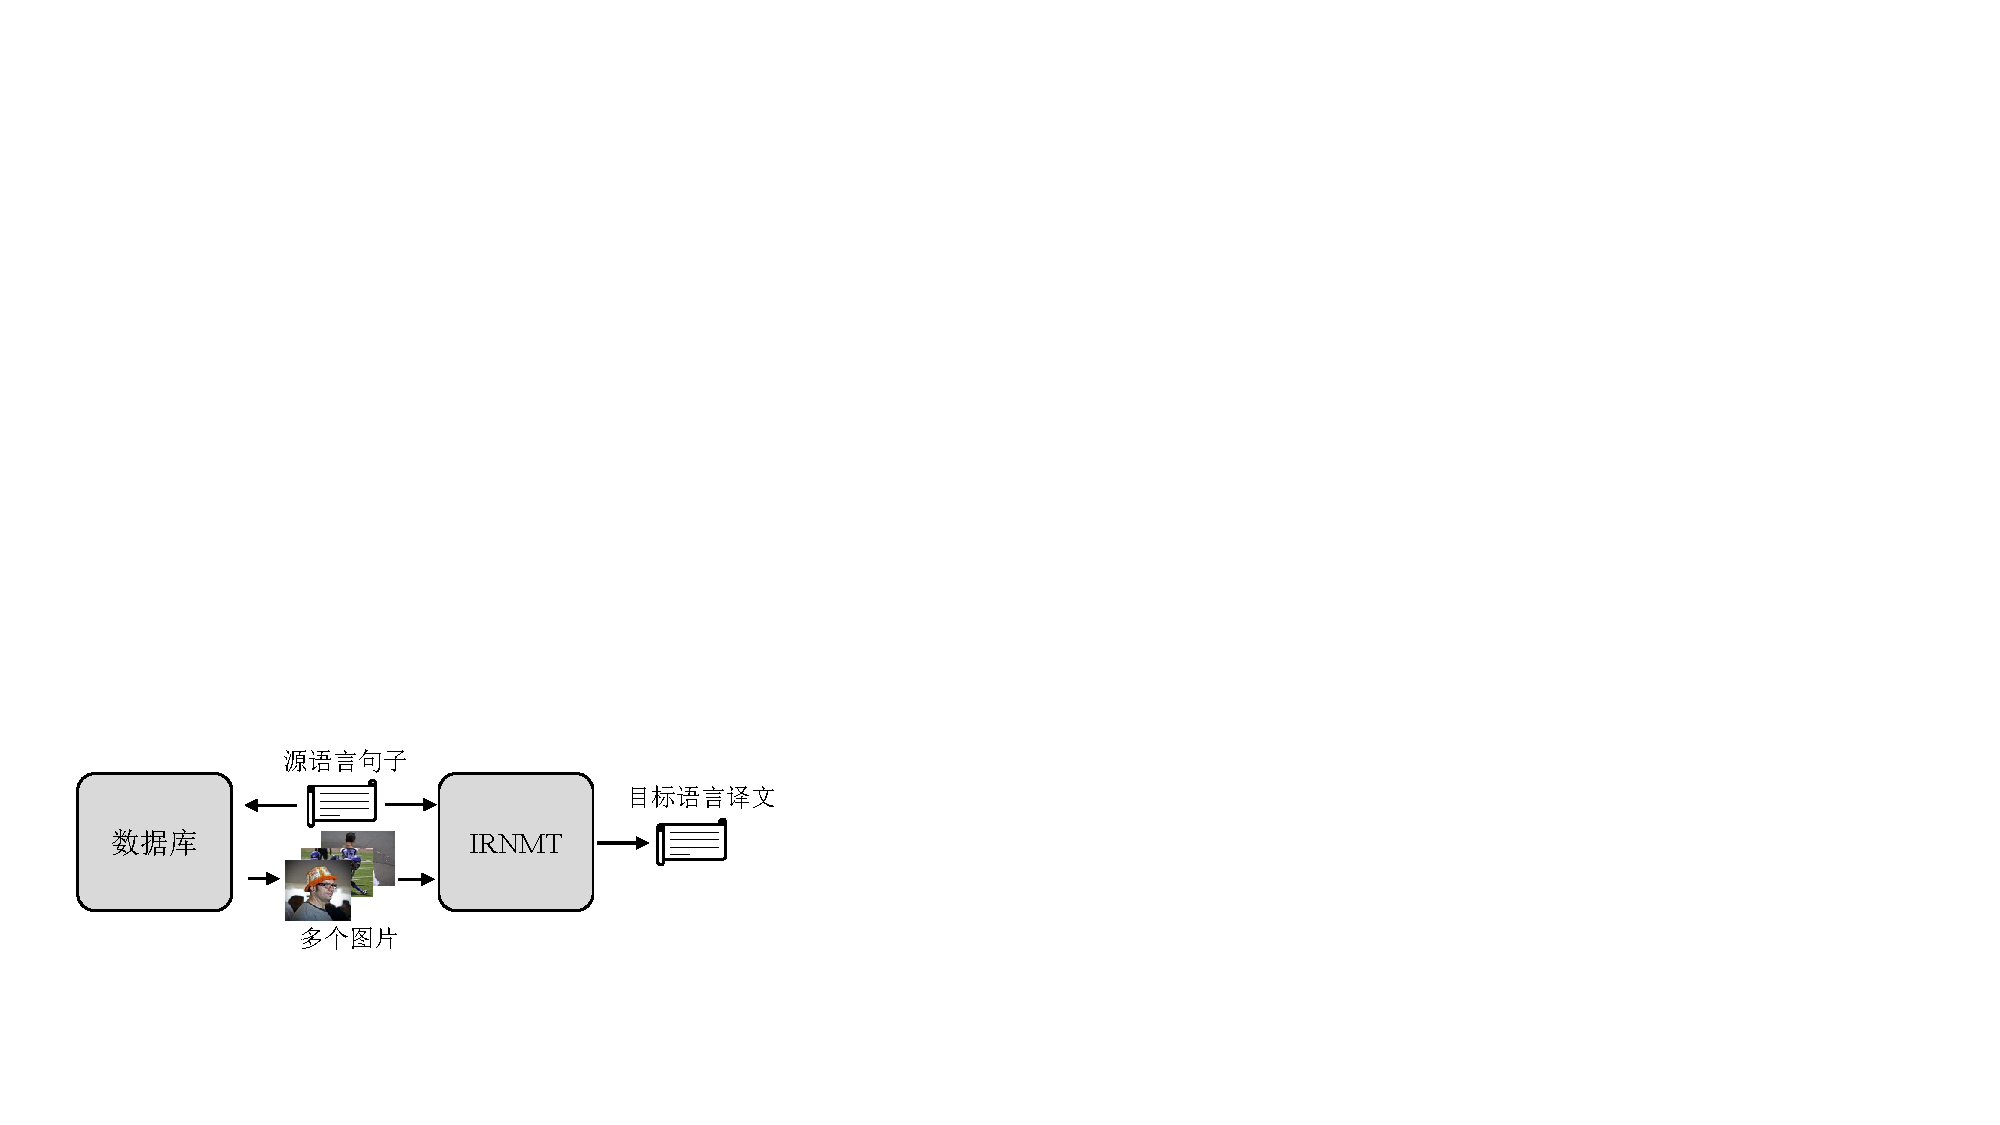
\includegraphics[scale=1]{Img/fig_2_irnmt.pdf}
    \bicaption{基于图片搜索的神经机器翻译}{Image-retrieval-based neural machine translation}
    \label{fig:2_irnmt}
\end{figure}
前两节所介绍的图片信息辅助式和图片信息增强式的神经机器翻译方法采用的都是与文本有着很强语义关系图片。因此,通常在图片描述的翻译任务上进行相关的研究与实验。本节的基于图片搜索的神经机器翻译(image-retrieval-based neural machine translation,IRNMT)与前面的方法区别在于该方法并不要求文本所描述的内容与图片内容完全一致。该方法采用与文本主题相关的搜索方法,从大规模单语语料或搜索引擎中收集相关图片。如图\ref{fig:2_irnmt}所示,为此类方法的研究范式示意图。文献\cite{118_DBLP:conf/iclr/0001C0USLZ20}首次提出在融合图片信息的神经机器翻译模型中增加搜索图片功能。该方法利用TF-IDF(term frequency-inverse document frequency)技术建立一个单词到图片的查找表,从这个查找表中可以获得图片的相关主题信息。在进行图片搜索之前,需要从源语言句子中提取出与句子内容相关的主题单词,然后根据主题搜索出若干个与该主题最相关的图片以此来获得所需要的图片信息。然后将这些图片的特征提取出来,最后传递给神经机器翻译模型用于辅助翻译生成。文献\cite{20_wu-etal-2021-good}在以上基于图片搜索的方法中测试图片信息是否能够为翻译带来提升。文献\cite{119_fang-feng-2022-neural}为了在搜索到更相关的图片,为翻译提供更准确的视觉信息,采用短语级别的图片作用方式,在搜索到图片后,需要提取出与主题相关的视觉目标,然后再进一步地在翻译中融合图片信息。
文献\cite{120_tang-etal-2022-multimodal}为了增加图片搜索的资源,并且使相关方法能够受益于一般的文本翻译任务,采用了基于商用搜索引擎的方案。

目前基于图片搜索的神经机器翻译方法的相关研究还处在初步阶段,基于搜索的方法的相关研究也在问答系统\cite{121_DBLP:conf/icml/GuuLTPC20}、对话系统\cite{122_DBLP:conf/emnlp/WestonDM18}、语言模型\cite{123_DBLP:conf/iclr/KhandelwalLJZL20}以及纯文本翻译\cite{124_DBLP:conf/aaai/GuWCL18}等任务中得到了应用。然而这类方法还存在着诸多问题需要进一步地解决,例如文本主题提取的准确性与覆盖性对图片搜索的影响,搜索获得图片与文本翻译内容的相关性对翻译带来的影响。
%这部分要强调使用完全对应图片的方案都很难使视觉信息起作用,那么采用搜索式的方式就更难了
%方法范式:与前面方法的最大不同点是否图文对应
%举例
%优点
%缺点

\subsection{基于图片信息的无监督神经机器翻译}
\begin{figure}[!htbp]
    \centering
    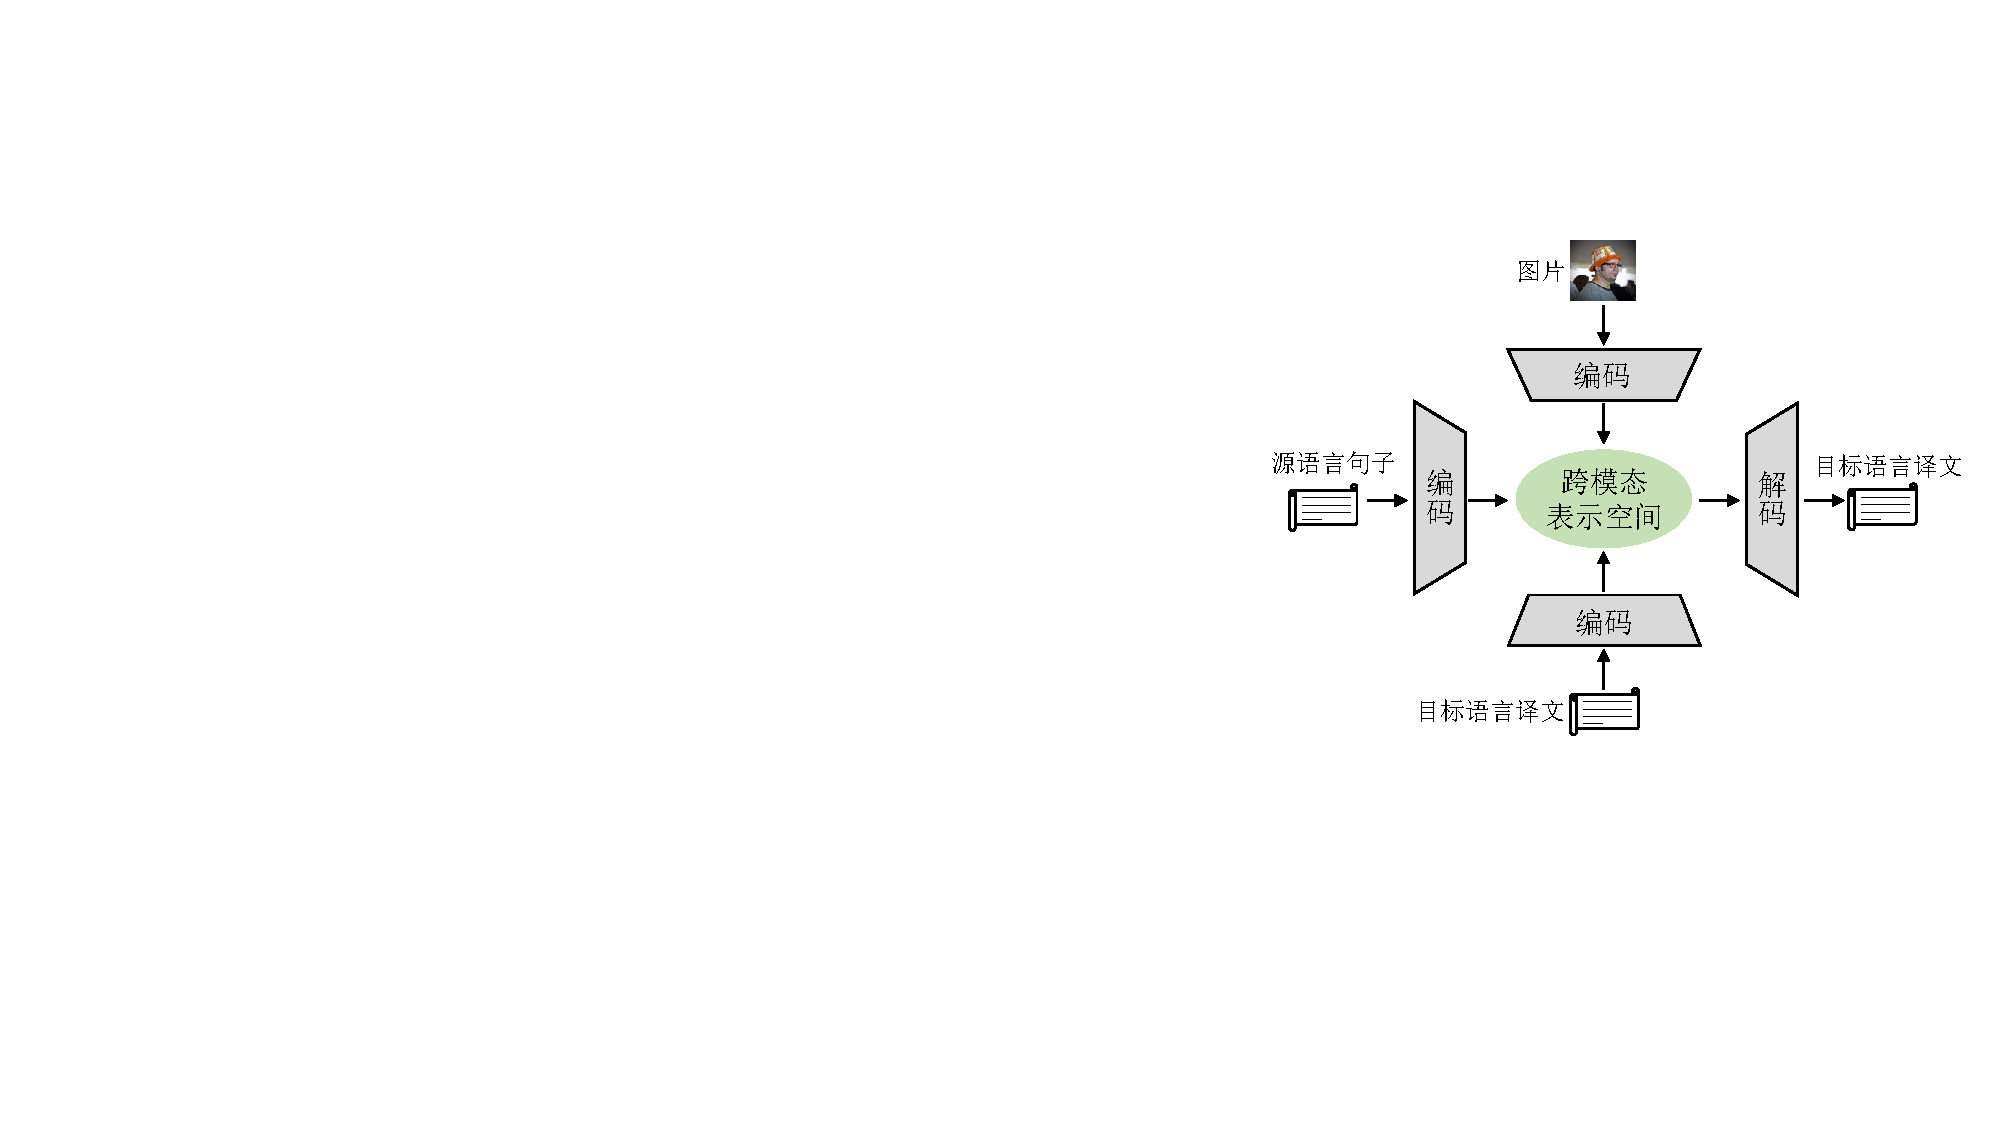
\includegraphics[scale=1]{Img/fig_2_iunmt.pdf}
    \bicaption{基于图片信息的无监督神经机器翻译}{Image-based unsupervised neural machine translation}
    \label{fig:2_iunmt}
\end{figure}
基于图片信息的无监督神经机器翻译(image-based unsupervised neural machine translation,IUNMT)是指利用图片作为语言桥梁,为零资源的翻译提供翻译支持的一类方法。零资源语言的翻译问题通常选择一个中间语言作为桥梁,通过将源语言翻译到中间语言,再将中间语言翻译到目标语言的方式,解决源语言到目标语言的翻译问题。然而,这种方法仍然需要源语言和目标语言到中间语言的平行翻译数据,而很多的低资源语言之间的翻译很难通过这种办法解决。考虑到人的语言可能分为多种,但人眼中的世界是统一的,并且社交媒体中包含了大量的单语的图文数据,所以选择视觉模态作为中间语言来完成零资源机器翻译任务是一个很好的选择。
文献\cite{115_saha-etal-2016-correlational}采用了中间语言方案解决源语言与目标语言之间没有平行的训练数据的问题。该方法选择图片作为中间语言,通过联合训练源语言到图片和图片到目标语言的生成模型,最终过得源语言到目标语言的翻译模型。
文献\cite{54_DBLP:journals/mt/NakayamaN17}同样将图片作为了中间语言,在训练过程中,将源语言、目标语言、和图片映射到一个统一的跨模态表示空间。
文献\cite{125_DBLP:conf/aaai/ChenLL18}将零资源的神经机器翻译模型的训练过程构建为一个多智能体交流游戏(multi-agent communication game)。每个智能体分别负责从图片中生成描述,以及从描述中生成目标语言译文的任务。两个智能体在两种任务的配合下完成源语言到目标语言的翻译建模。
文献\cite{126_DBLP:conf/cvpr/SuFBKH19}采用降噪模型的训练方式构建中间语言与源语言和目标语言的编码器和解码器,在联合使用编码器和解码器的情况下实现源语言到目标语言之间的翻译。
文献\cite{55_DBLP:conf/ijcai/ChenJF19}认为图片中包含太多与待翻译句子以及译文不相关信息,直接作为句子级语义单位的中间语言会引入大量噪音,因此将图片先应用到词的翻译,在通过迭代生成伪平行句对的方式,逐步实现句子级的翻译。
文献\cite{127_huang-etal-2020-unsupervised-multimodal}同样通过图片生成伪平行句对的方式逐步训练翻译模型。



